% !TEX root = ../maturaarbeit.tex
\chapter{Core concepts of Reinforcement Learning}\label{chap:theory}
\section{What is Reinforcement Learning?}\label{sec:RL}
\noindent
Throughout our daily lives we navigate our surroundings, handle social situations and tackle complex tasks. In doing, so we take those actions, based in experience and intuition, which we believe to have the best outcome. We might take these abilities for granted, given how natural they are to us. However, at some point we had to obtain these skills, so essential in managing our day to day, many through simple trial and error. Reinforcement Learning (RL) seeks to formalize the process of figuring out how to behave based on seeing what produces desirable results and what does not, and adjusting our future actions accordingly. 

\noindent
\\ Reinforcement Learning is a discipline of machine learning \cite[p. 1]{sutton_reinforcement_2018}, an incredibly broad field which is focused on the self-improvement of computer algorithms by processing data and experience. As such it is at the interface between the natural, to us intuitive concept of learning, and the rigid and numerical world of computer programming and mathematics \cite[p. 4]{sutton_reinforcement_2018}. Thus, to be able to understand how this learning process works, and to be able to quantify and formalize it, it is essential to introduce generalizable concepts that accurately describe its components. 

\subsection{Illustrative Example: Card game UNO}\label{subsec:UNO}

\begin{figure}[ht]
    \centering
    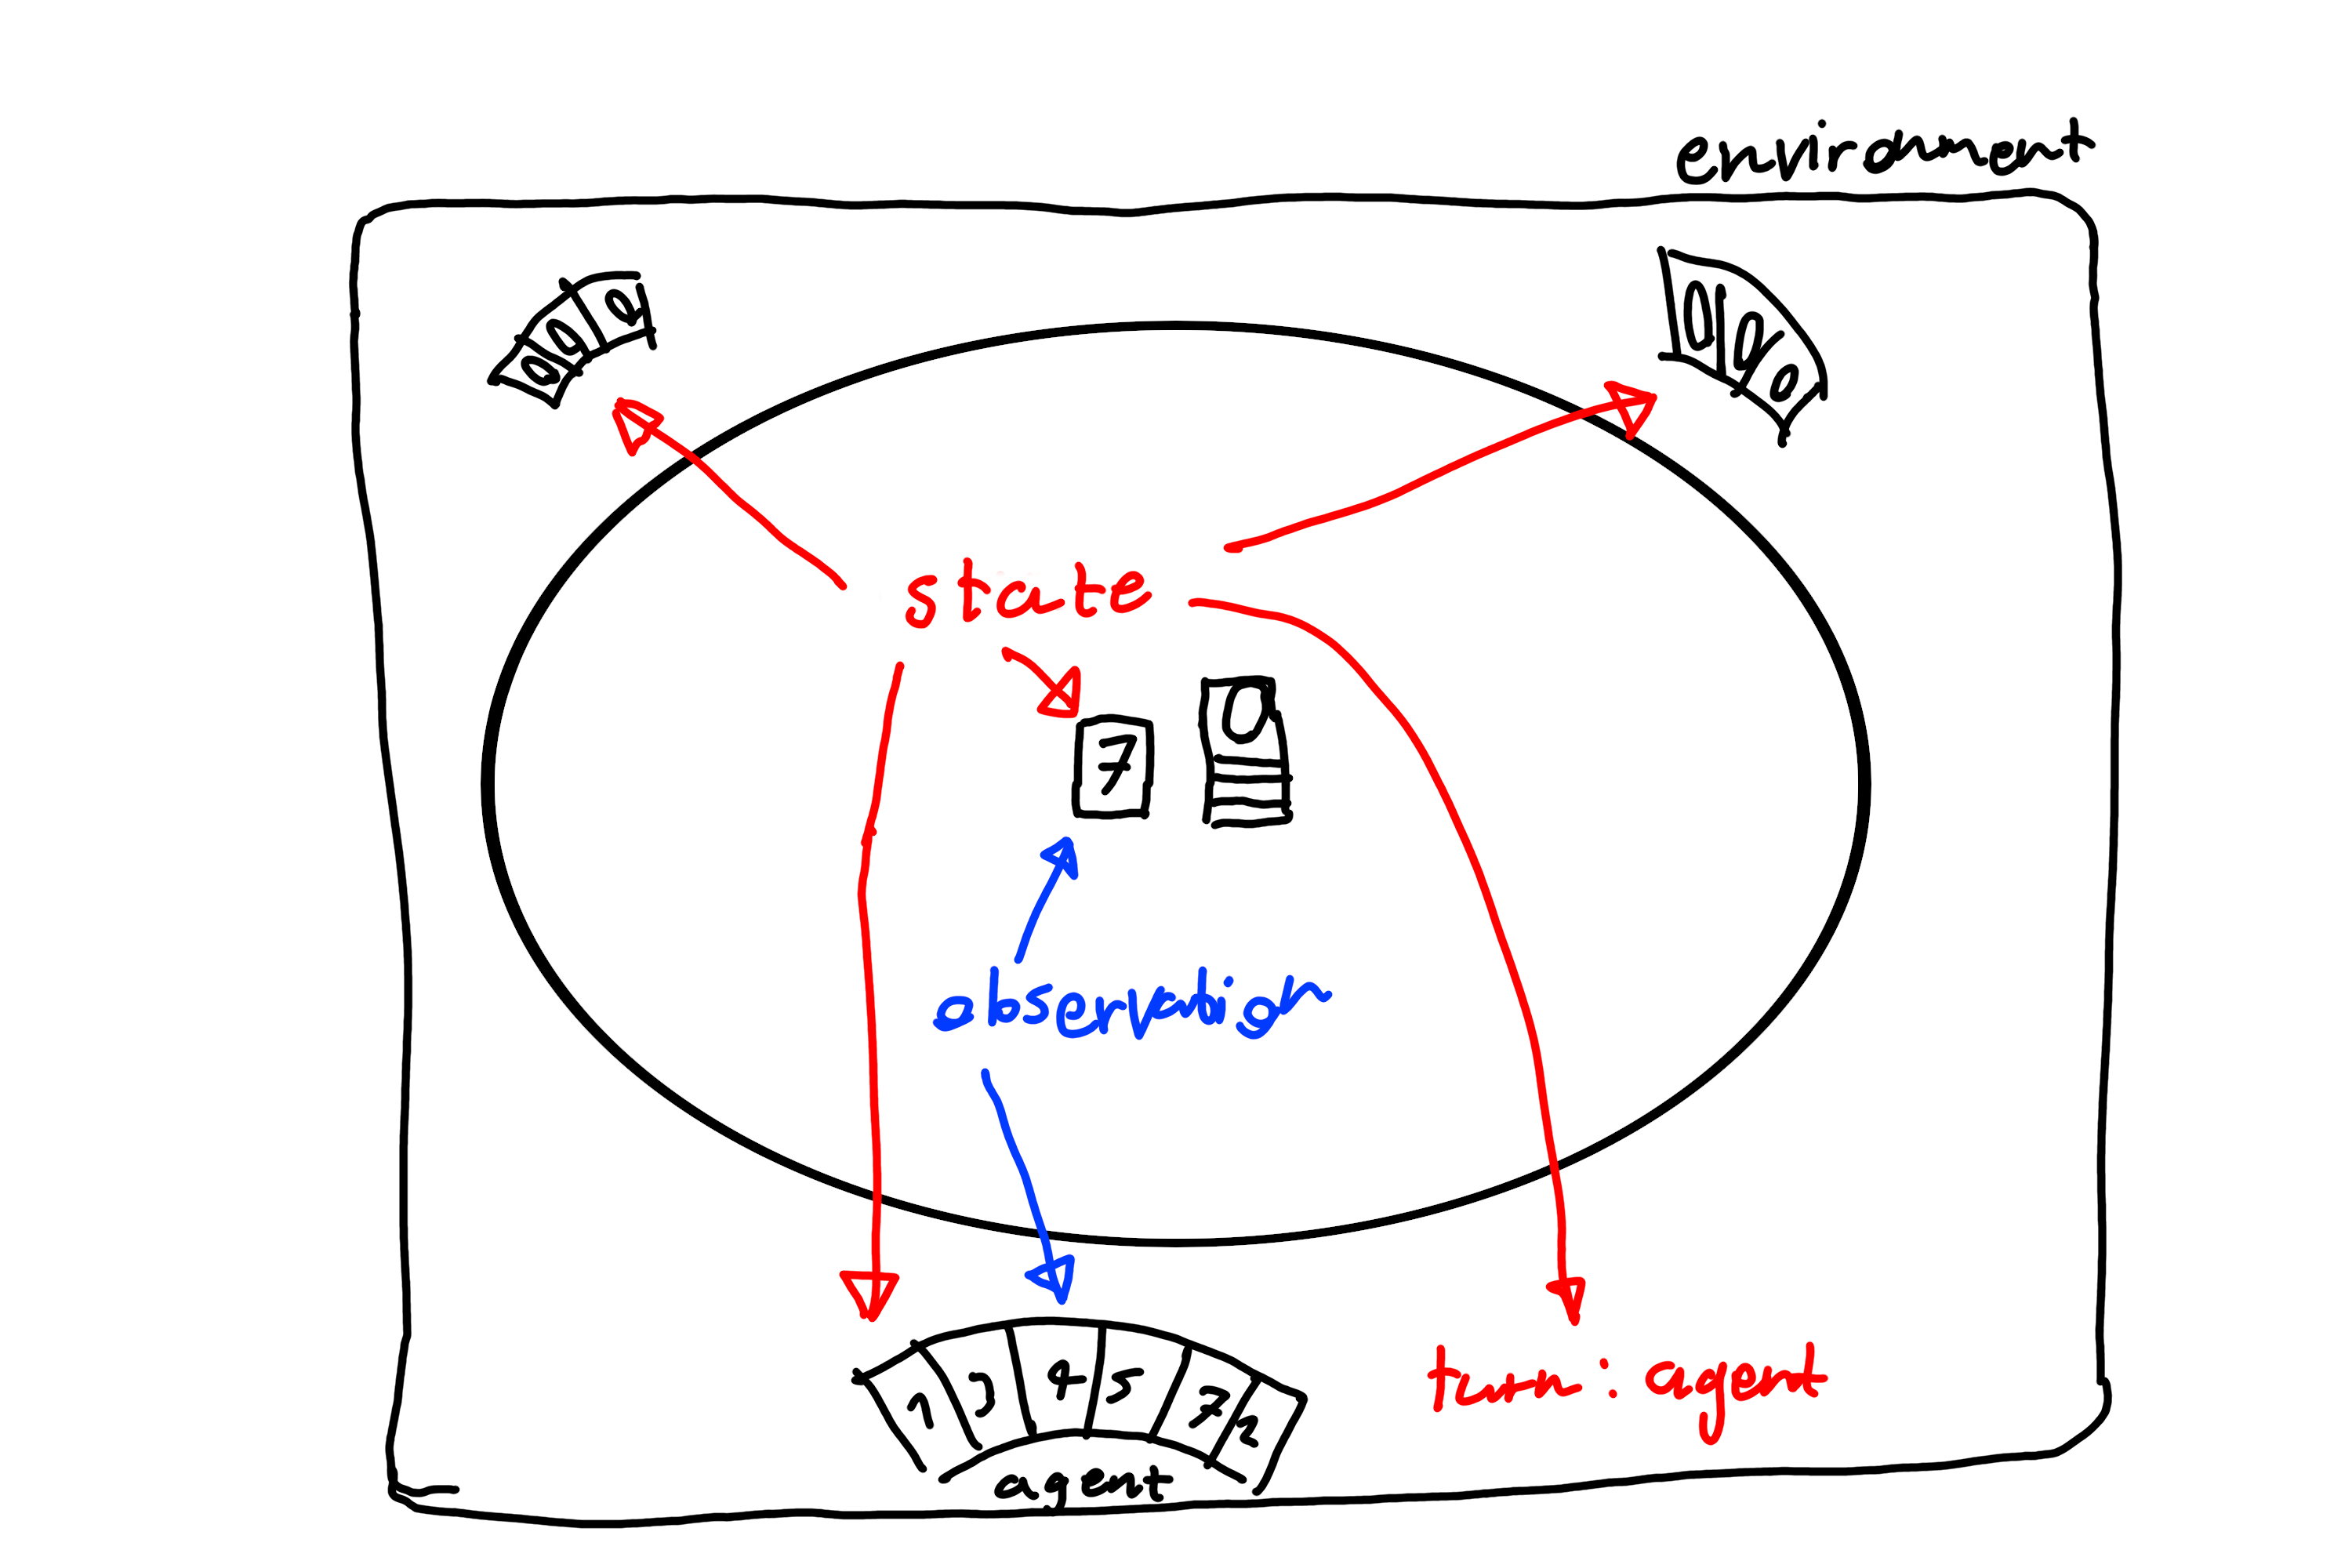
\includegraphics[width=\linewidth]{figures/UNO.png}
    \caption{UNO environment in the context of RL}
    \label{fig:UNO}
\end{figure}

\noindent
To do so, consider the example of playing the popular card game “UNO”. The \textit{objective} of the game is to rid oneself of the cards on your hand while preventing the other players from doing so. We can label the game as an \textit{environment}. This environment contains all the players, the cards and also what rules the game follows. It  can be in any arbitrary \textit{state s}. A state of an environment describes the arrangement of all components belonging to the it, in this case the hands of the players, who's turn it is, what cards are on which pile and what order they are in. Notice that the environment contains a lot of information which the player, in Reinforcement Learning called an \textit{agent}, an actor in the environment, does not know about. However, the actor can \textit{observe} the environment and thus gain a reasonably accurate representation of it’s state. Say it is the agents turn. Based on its \textit{observation} the agent can take \textit{action a}, the agent can play any of the cards on its hand, or pick one up. It might not be able to play every card or none at all, and it attempting to take an action which the rules of the environment disallow will result in the same state, where it is the agents turn, but the other players will have told the agent that their action is invalid, in other words the environment will have given it a negative \textit{reward signal}. Based on the \textit{reward} the agent then can update its way of acting to produce a different action next time. Thereby the reward \textit{reinforces} the desired behaviour, it is a \textit{reinforcement}. The way of acting of an agent in a state given an observation of that state, is called a \textit{policy}, commonly denoted as $\pi$. The agent can follow a policy to obtain an action, given a state.
\newline
For the sake of brevity, unless the distinction is relevant, I am going to equate observation and state moving forward. Much more expansive definitions going in to the nuances of these concepts can be found in the book \textit{Reinforcement Learning, An introduction} by Richard Sutton and Andrew Barto. \cite{sutton_reinforcement_2018}

\subsection{Why chose Reinforcement Learning over other approaches?}\label{subsec:Why_RL}
In a simple example like UNO Reinforcement Learning might indeed not be the best approach. All the rules of UNO are known to the player, and the set of all possible states is fairly limited. The player also knows about all the cards in the game and thus an algorithm which takes in all the information available to the player, computes the action which has the highest probability of leading to victory, and picks it. However, this approach requires full knowledge of how the environment operates \cite[p. 8]{sutton_reinforcement_2018}. This quickly becomes unfeasible as the environment grows more complex. Reinforcement Learning lets us generate high quality solutions in uncertain environments based on a reward signal and the goal it ultimately describes \cite[p. 03]{sutton_reinforcement_2018}. Another approach which might come to mind as an obvious solution would be to simply mimic the behaviour of an optimal, or close to, agent. However, this again is impractical as such an agent might simply not exist or generating sufficient examples can be tedious. As stated in Reinforcement Learning, An Introduction: “In uncharted territory—where one would expect learning to be most beneficial, an agent must be able to learn from its own experience.” \cite[p. 02]{sutton_reinforcement_2018} Here it is important to keep in mind that uncharted environments for machines are vastly different from those of a human. There might very well be uncountable examples of brewing a coffee, but possibly non of how to power a series of motors based on a video feed in order to achieve that same goal.

\section{Finite Markov Decision Processes, a mathematical framework for Reinforcement Learning}\label{sec:MDP} % NOTE: THESE ARE ALL REFERENCES TO THE BOOK
I this section I will introduce Finite Markov decision processes (MDPs) which serve as a formalization of sequential decision making. Environments which can be formulated as finite MDPs are what Reinforcement Learning is trying to solve. They are finite because the sets $\mathset{S}, \mathset{A}, \mathset{R}$ of all states, actions, and rewards are all finite. I will illustrate and apply the concepts in this section using the Grid-World environment. It serves as a particularly convenient example since in it, the state of the environment is fully described by the agents position. This allows for simple computation and visualization. 

\subsection{Sequential decision making}\label{subsec:sequential_decision_making}
In an MDP the agent and environment continually interact. This creates a loop where the agent selects an action, the environment transitions in to a new state $S_{t+1}$ and gives the reward $R_{t+1}$. Based on this new state, the agent selects another action. This may repeat forever. However, importantly it does not require $S_{t+1}$ to be novel, as this would render a finite set of states impossible. It is just the state which the environment transitions to next, however it may be the same state as one which was previously visited, the environment may even transition back to itself. This is possible because all possible futures solely depend on that state, else it would not fully describe the environment.

\begin{figure}[h!]
    \centering
    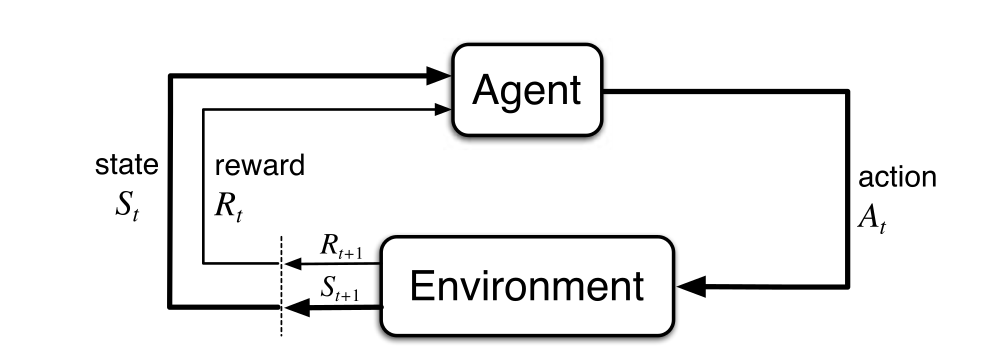
\includegraphics[width=0.7\linewidth]{figures/agent_environment_interaction_loop.png}
    \caption{Agent Environment Interaction Loop as presented in \citepg{48}}
    \label{fig:agent_env_inter}
\end{figure}

\noindent
This interaction can be broken up in to time-steps. At each time-step the agent is given the current state of the environment and receives a reward based upon the previous state and action taken. thus at time-step $t$ there exists a state, action and reward $S_t, A_t, R_t$ , each of these is an element of their respective finite sets presented above. \citepg{48}. Since the agent environment interaction is sequential, a sequence, or in Reinforcement Learning \textit{trajectory} written as $\tau$, arises, where each subsequent state, action, reward triple is of time-step $t+1$. \citepg{48}

\begin{equation}\label{MDP:trajectory}
    \Tau = S_0, A_0, R_1, S_1, A_1, R_2 \dots
\end{equation}
\centerline{\small\textit{from \citepg{48}}}

\noindent
\\ In an \ita{episodic} environment, an environment that ends at some terminal time-step $T$, a trajectory has a terminal state $S_T$ and reward $R_T$. The notion of a terminal action does not make sense since the environment terminates at $T$, any action taken would not have an effect, and the action which proceeds $S_T$ is $A_{T-1}$. Continuous environments, which episodic ones are a special case of, do not terminate, learning has to be done concurrently with exploring the environment, or at set intervals. This presents a further set of challenges. I will cover some of those herein, however my focus will lie with the episodic case, as it is most relevant to my work.

\subsubsection{Illustrating in Grid-World}\label{subsubsec:grid_world_trajectory}
The Agent starts at a starting position, here the bottom left corner, it is in the first state, $S_0$. A black field on the grid signifies its inaccessibility. The episode is terminated if the agent reaches the upper right corner, or the field below it. The rewards are not yet displayed here to avoid clutter, they will be discussed in the next section.

\begin{figure}[h!]
    \centering
    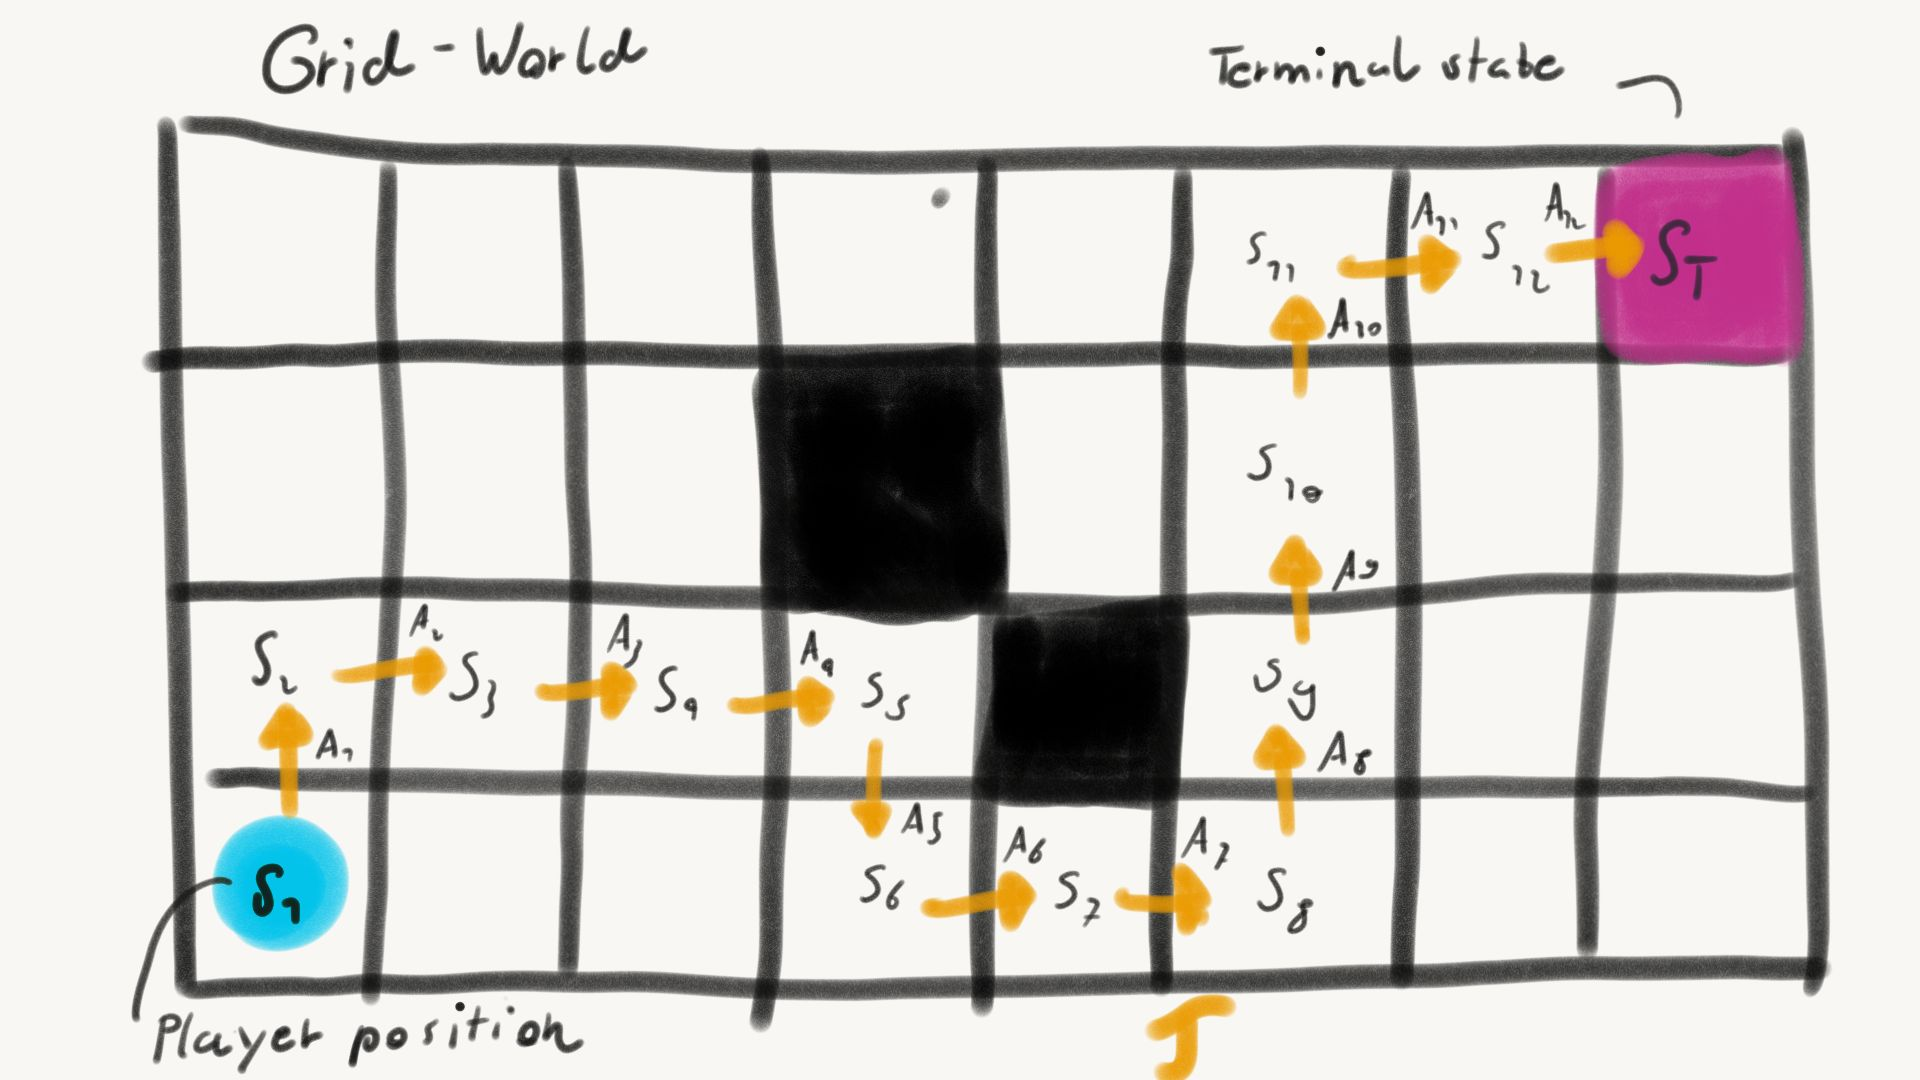
\includegraphics[width=0.7\linewidth]{figures/Grid_world_trajectory.jpeg}
    \caption{The Grid World Environment}
    \label{fig:grid_world}
\end{figure}

The agent then moves through the states and therein generates a trajectory. The representation of that trajectory overlaid on to the grid, works in this case because the agents position fully describes an environment state. At each time-step the agent can choose to move up, down, left or right. Knowing a trajectory mainly becomes useful in improving the agents performance. If a full episode is known at evaluation, an action taken can be put in to the context of everything which happened after it. Knowing what something led to in the future is obviously useful in evaluating it.

\subsection{Defining the Agents goals in a MDP}\label{subsec:goals}

The agent selects actions based on state information and and receives rewards as feedback for its previous action. It intuitively follows that the goal of the agent is to maximize the reward received. However based on that model the agent changes its policy purely based solely on the reward it immediately receives after an action, in other words it is only aware of the correlation between an action and its immediate consequences. Needless to say, inability to plan for long term reward presents a problem. The \ita{Return} $G$, which is defined as follows, presents one possible solution for this issue.

\begin{equation}\label{MDP:return}
    G_t \doteq R_t + R_{t+1} + R_{t+2} \dots + R_T
\end{equation}
\centerline{\small{\ita{\citepg{54}}}}

\noindent
\\ By the above the return describes the sum of all rewards up until the end of the episode. This presents some issue if the environment is continuous, since there is no final time-step. To remedy this \ita{discounting} is introduced. \citepg{55} The discounted return be expressed as the sum to infinity:
\begin{equation}\label{MDP:discounted_return}
    G_t = \sum_{k=t}^{\infty} R_{t+k+1} * \gamma ^k 
\end{equation}
or recursively as
\begin{equation}\label{MDP:recursive_discounted_return}
    R_{t+1} + \gamma *G_{t+2} \mathrm{\ where\ } 0 \leq \gamma \leq 1
\end{equation}
\centerline{\small{\ita{\citepg{55}}}}

\noindent
\\ Discounting has some other advantages as well. Caring about all future outcomes equally might not always be the behaviour sought in an agent. According to \citepg{57} this generalization can be applied to the episodic case by defining the environment to transition from the final state $S_T$ to itself and to only ever give a reward of 0, thus not affecting the return of any given time-step in the episode. The following illustration from \citepg{57} visualizes this approach neatly.

\begin{figure}[h!]
    \centering
    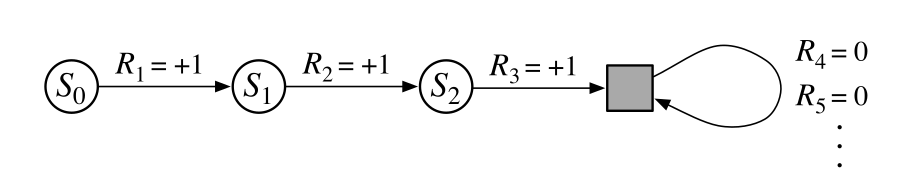
\includegraphics[width=0.6\linewidth]{figures/unified_notation_from_book.png}
    \caption{The episodic case in unified notation as illustrated in \citepg{57}}
    \label{fig:unified_continuous_episodic_return}
\end{figure}

\noindent
\\ If the return is used to update the agents policy, the agents "cares" about future rewards as well. Therefor such an agent, given sufficient training, will not take the action which yields maximal immediate reward, but the rather that which gives maximal return, thereby plan for the future. Given this, an additional purpose of the discount factor $\gamma$, is to balance an agents planning for future reward and seeking immediate results. One might be tempted to set the discount factor to one, however this muddies the correlation between an action and its results thus possibly slowing the learning process. It is another hyper parameter that needs to be set and which greatly affects the proficiency of an agent. The effects of this in the grid-world environment are clearly visible here:

\begin{figure}[h!]
    \centering
    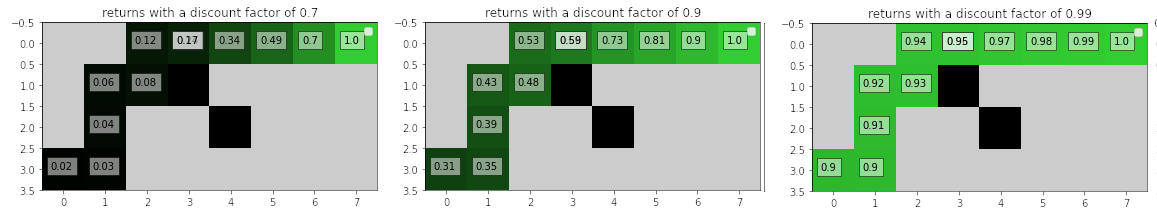
\includegraphics[width=\linewidth]{figures/grid_world_discount_factors.png}
    \caption{Returns for each time step in an episode for different discount factors}
    \label{fig:grid_world_discount_factors}
\end{figure}

\noindent
\\ The only reward the agent receives here occurs on the final time-step, and has a magnitude of 1. Notice how quickly the return decays with even a discount factor 0.9. This makes the agent quite short sighted. Due to this small discount factors often do not make sense. A discount factor of 1.0 is viable as well. As with many parameters, it should be tailored to the problem at hand.

\noindent
\\ The agent seeking to maximize the return, that in a sense being its \ita{goal}, also has some important implications for defining the rewards received by the agent. Rewards should be proportional to the "goodness" of an action which lead to them and since they are the only information the agent can learn from should also not be too sparse. The problem of dealing with environments which give sparse reward is a large hurdle in modern day RL, some solutions to this are addressed in \citepg{491}. In such environments it turns out to be useful to modify the rewards received by setting baselines, creating "intrinsic rewards", those could for example be rewards for exploring the environment and many others. 

\subsection{Environment Dynamics}\label{subsecec:env_dynam}

Another component in the agent environment interaction are the \ita{dynamics} of the environment. An environment does not have to be \ita{deterministic} in an MPD. This means that a specific action does not have to have only one predetermined outcome. Rolling a die might be an action, the outcome can however not be know prior to taking it. A given action can have multiple possible subsequent states and rewards, however the distribution of these must be well defined. in \citepg{48} this gives rise to the following pair of equations:

\begin{equation}\label{MDP:prob_dist:0}
    p(s', r |s, a) \doteq Pr\{ S_t=s', R_t=r | S_{t-1}=s, A_{t-1}=a\}
\end{equation}
where 
\begin{equation}\label{MDP:prob_dist:1}
    \sum{s \in \mathset{S}}^{}\sum{r \in \mathset{R}}^{}  p(s', r |s, a) = 1 \mathrm{\ for\ all\ } s \in \mathset{S}, a \in \mathset{A}(s) 
\end{equation}
\centerline{\small{\ita{taken from \citepg{48, 49}}}}

\noindent
\\ In effect these define a probability distribution over future states and rewards given a state and an action. To give a better intuition it is worth looking at the previous Grid-World example again. For this assume that the agent is at state $S_9$. A graph of the transition probabilities at that state might be graphically illustrated as follows:

\begin{figure}[h!]
    \centering
    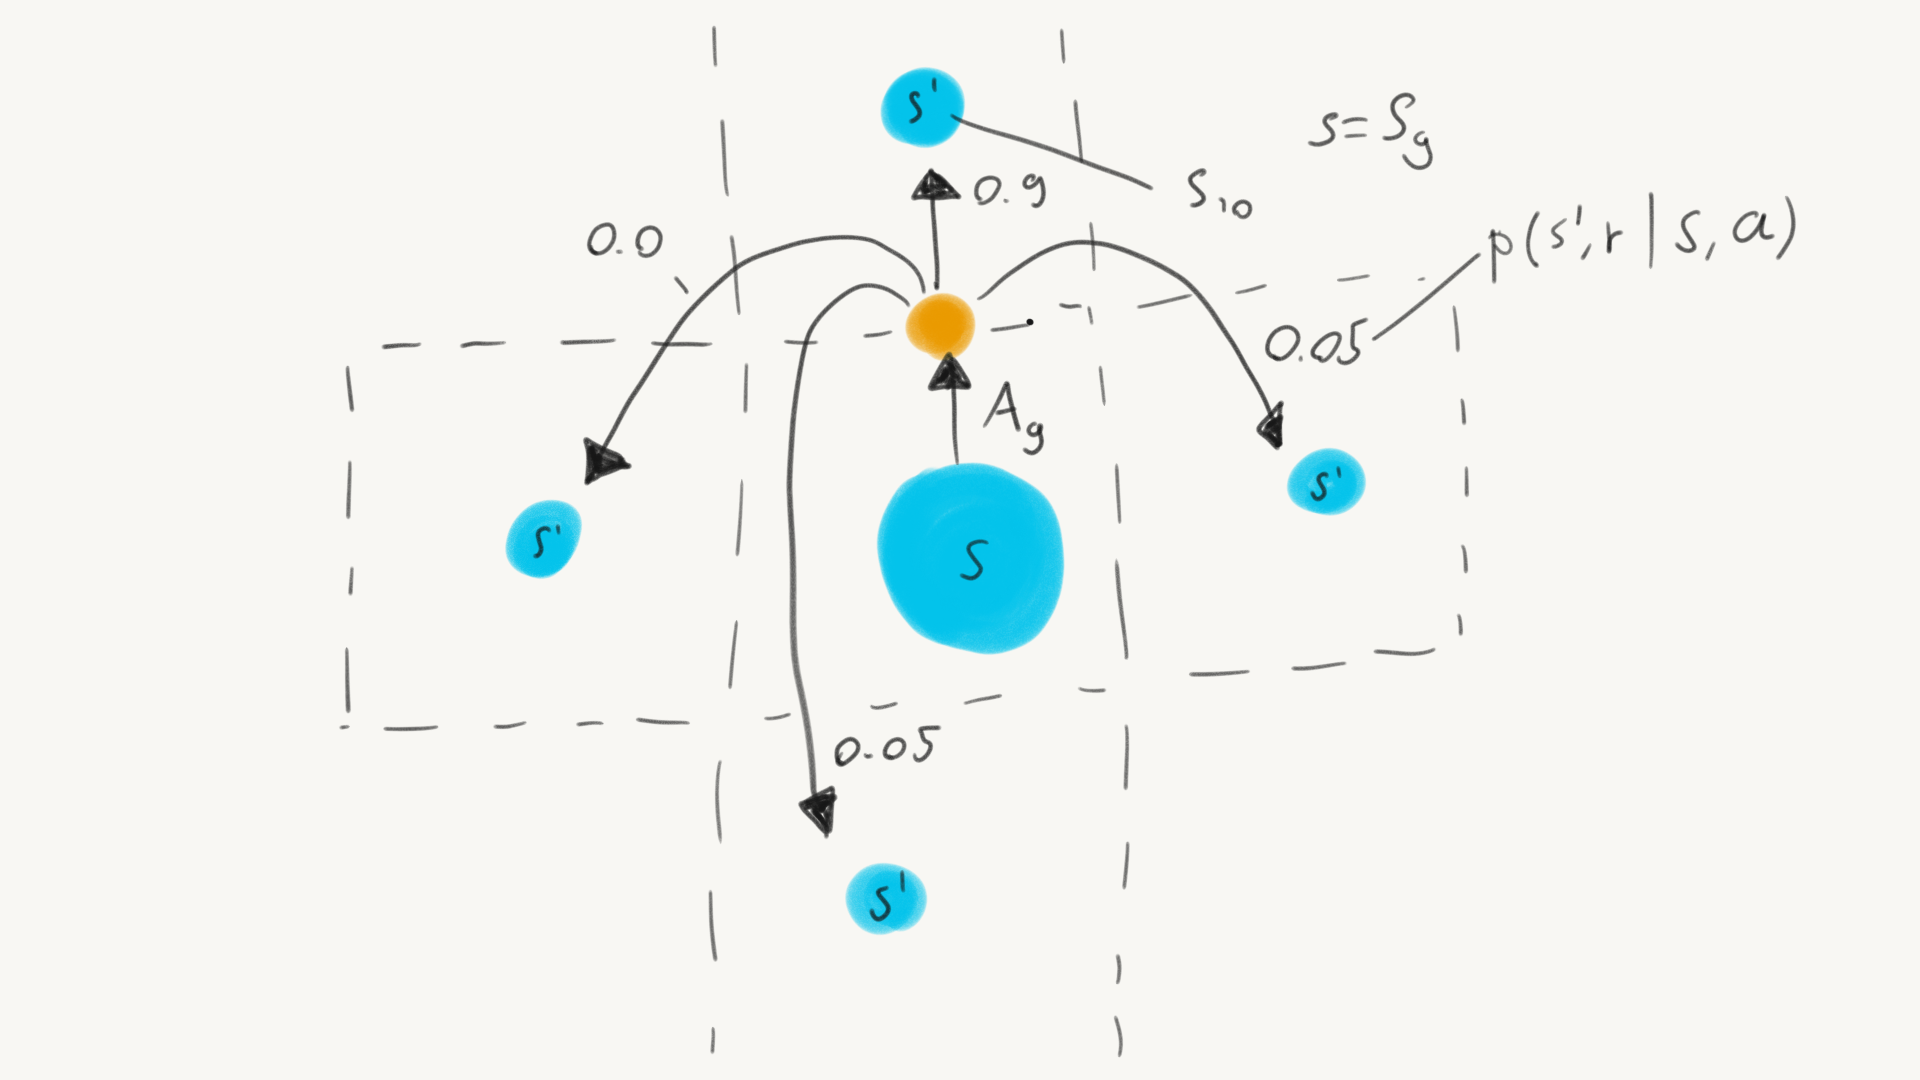
\includegraphics[width=0.5\linewidth]{figures/mdp_dynamics.png}
    \caption{Environment dynamics of Grid-World at in an episode at state $S_9$}
    \label{fig:mdp_dynamics}
\end{figure}

\noindent
\\ Starting at state $S_9$ the agent takes action $A_9$, up, (here in orange). Then it has a probability of 0.9 of ending up in the field above the one its in. However it might also end up in the field below or to the right, with an equal probability of 0.05. In the case of Grid-World this might be interpreted as the agent tumbling, however more generally they just describe uncertainty of outcome in an environment when an action is taken.

\subsection{Policies in a MDP}\label{subsec:policies}
Moving forward it is important to understand what policies are mathematically. So far it has been established that policies are the way in which an agent behaves in an environment, the actions they give can have a factor of randomness and in a good policy the the action taken most likely depends on the current state. This gives rise to the policy as a simple function which takes a state and produces a probability distribution over the set of actions. This distribution can be discrete or continuous and is not restricted to a single axis. An action can simply be obtained from a policy by sampling from it. This is outlined in \citepg{58}, where $\pi(a|s)$ is defined as the probability of $a$ given $s$ under $\pi$. This also allows for writing the transition probabilities for $s$ to $s'$ as $\pi(a|s) \cdot p(s', r|s, a)$. The product of the probability of choosing an action under a policy and the the probability of that state occurring given $s, a$. This becomes relevant in \ref{sec:policy_gradient} where I present the foundation for the main solution method used in this thesis.

\subsection{Value Functions as a measure of Policy  performance}\label{sec:value_functions}
In reinforcement learning it is often useful to have a measure how good it is for an agent to be in some state given its current way of acting, its policy. As stated in \citepg{58} the "goodness" of a state $s$ under some policy $\pi$ is described by the state value function $v_\pi(s)$. Mathematically this value function is:

\begin{equation}\label{state_value_function}
    v_\pi(s) \doteq \mathbb{E}_\pi[G_t | S_t=s] = \mathbb{E}_\pi[\sum_{k=0}^{\infty} y^k R_{t+k+1}|S_t=s] , \mathrm{\ for\ all\ } s \in \mathset{S}
\end{equation}
\centerline{\small{\ita{\citepg{58}}}}

\noindent
\\ Notice that this applies to the unified discounted case. This value function under a policy describes what return or discounted sum of future rewards, following the policy $\pi$. Since the rewards, and in turn the return, is what reinforcement learning seeks to maximize, this value function can be used as a measure of the policy starting at state $S_t$. Since our example of grid-world is very limited in scope, an estimate of the value function can simply be found be repeatedly sampling from the policy $\pi$ computing the return, and updating a value in a table corresponding to the state with the discounted difference between the actual return and its expectation. this generates a decent estimate of the expectation of $G_t$.

\begin{figure}[h!]
    \centering
    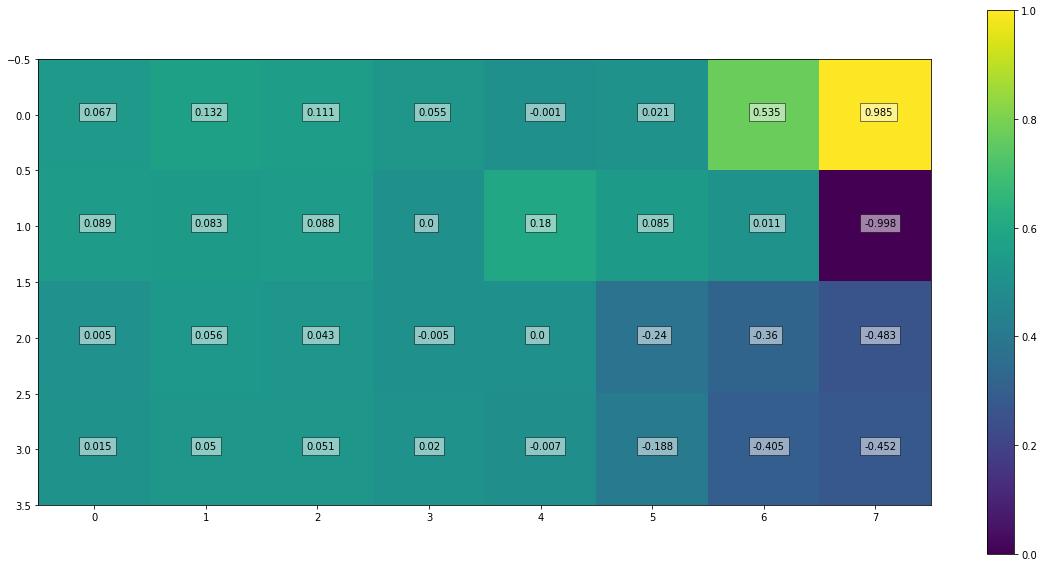
\includegraphics[width=0.6\linewidth]{figures/state_values_under_pi.png}
    \caption{Estimated Value Functions for each state}
    \label{fig:value_functions_grid_world}
\end{figure}

\noindent
\\ These are the results of estimating the value functions for all states, using random policy. One interesting feature which can be seen here is the low expected return for all states in bottom right corner. This most likely stems from the fact that a random agent will likely end up in the terminal state which gives a reward of -1. This tabular method of estimating value functions under $\pi$ works well enough in Grid World. However it falls apart rather quickly once the number of states increase, as already is the case once the environment is even slightly more complex. This can already be seen in the child's game Tic-Tac-Toe, which has 9 fields, 3 possible values per field and 2 players who's turn it could be. this leads to $3^9 * 2$, almost 40'000 possible permutations of the environment. Value functions can be used to during training of an agent to give context for the return received from an environment and in some cases even directly offer solutions to it, these however exceed the scope of this thesis. This makes them undeniably useful. Because of this function approximators, which I will elaborate on in chapter \ref{chap:neural_networks}, are often used to estimate state-value functions. There also exist action-value functions which take an action and are the expectation of the return under a policy if the given action is taken in said state. Action value functions are denoted as $q(s, a)$ and form the basis of Q-Learning. This method of solving an MDP is detailed in various variants in \cite{sutton_reinforcement_2018}, I will not further elaborate on them here, they are not the focus of my work.
